% 'Notas de aula não oficiais de MS650 e F620' (c) 2012, 2013 by Raniere Silva
% <ra092767@ime.unicamp.br>
%
% 'Notas de aula não oficiais de MS650 e F620' is licensed under a
% Creative Commons Attribution-ShareAlike 3.0 Unported License.
%
% You should have received a copy of the license along with this
% work.  If not, see <http://creativecommons.org/licenses/by-sa/3.0/>.

% Este arquivo inclui o conteúdo de:
%
% * M2S12-15.pdf
% * M2S12-16.pdf

\chapter{Transformadas Integrais: Outros Exemplos e Aplicações}
Uma transformada integral é uma transformação que leva uma função $f(x)$ em uma
função $F(y)$ através de
\begin{dmath*}
  F(y) = \int_{\alpha}^{\beta} K(x, y) f(x) \vi{x}
\end{dmath*}
Chamamos $K(x, y)$ de núcleo da transformada. Podemos ainda, no caso de
considerarmos variáveis complexas, tomar a integral acima ao londo de um caminho
no plano complexo. Os exemplos que já vimos são:
\begin{enumerate}
  \item Fourier: $\alpha = -\infty$, $\beta = +\infty$ e $K(x, y) = \exp(i x
    y)$.
  \item Laplace: $\alpha = 0$, $\beta = +\infty$ e $K(x, y) = \exp(- x y)$.
\end{enumerate}

Existem, é claro, vários outros exemplos mais ou menos importantes dependendo do
contexto considerado. Vamos a seguir ver alguns outros exemplos que tem a sua
importância particular.

\section{Transformada de Mellin}
Vamos considerar o par de transformadas de Fourier:
\begin{dgroup*}
  \begin{dmath*}
    A(w) = \int_{-\infty}^{+\infty} a(t) \exp(i w t) \vi{t} \condition{$\alpha <
    \Im(w) < \beta$},
  \end{dmath*}
  \begin{dmath*}
    a(t) = \frac{1}{2 \pi} \int_{i \gamma - \infty}^{i \gamma + \infty} A(w)
    \exp(- i w t) \vi{w} \condition{$\alpha < \gamma < \beta$}.
  \end{dmath*}
\end{dgroup*}
Vamos fazer a mudança de variáveis: $p = i w$ e $x = \exp(t)$. Assim:
\begin{dgroup*}
  \begin{dmath*}
    F(p) = A(-i p)
    = \int_{0}^{\infty} a(\ln x) x^p \frac{\vi{x}}{x}
    = \int_{0}^{\infty} a(\ln x) x^{p - 1} \vi{x}
    - \int_{0}^{\infty} f(x) x^{p - 1} \vi{x},
  \end{dmath*}
  \begin{dmath*}
    f(x) = a(\ln x)
    = \frac{1}{2 \pi} \int_{C - i \infty}^{C + i \infty} A(-i p) x^{-p}
    \frac{\vi{p}}{i}
    = \frac{1}{2 \pi} \int_{C - i \infty}^{C + i \infty} F(p) x^{-p}
    \frac{\vi{p}}{i} \condition{$\alpha < \Re(p) < \beta$}.
  \end{dmath*}
\end{dgroup*}
Definimos assim a Transformada de Mellin,
\begin{dmath*}
  F(p) = \int_{0}^{\infty} x^{p - 1} f(x) \vi{x}
\end{dmath*}
e a Transformada de Mellin inversa,
\begin{dmath*}
  f(x) = \frac{1}{2 \pi i} \int_{C - i \infty}^{C + i \infty} F(p) x^{-p}
  \vi{p}.
\end{dmath*}

\begin{exem}
  Considere a função $f(x) = \exp(-\alpha x)$ para $\alpha > 0$. Então
  \begin{dmath*}
    F(p) = \int_{0}^{\infty} \exp(-\alpha x) x^{p - 1} \vi{x}
    = \frac{1}{\alpha p} \int_{0}^{\infty} \exp(-y) y^{p - 1} \vi{y}
    = \Gamma(p) / (\alpha p).
  \end{dmath*}

  Para calcular a transformada inversa devemos lembrar que a função gama,
  $\Gamma(p)$, possui pólo simples em $p = 0, -1, -2, -3, \ldots$
  \begin{figure}[htb]
    \centering
    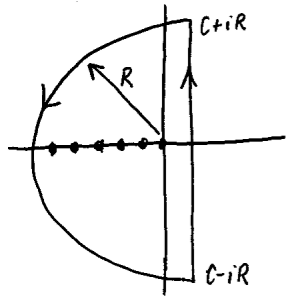
\includegraphics{figuras/15-0}
  \end{figure}
  Então
  \begin{dmath*}
    f(x) = \frac{1}{2 \pi i} \int_{C - i \infty}^{C + i \infty} x^{-p}
    \frac{\Gamma(p)}{\alpha p} \vi{p}
    = \frac{1}{2 \pi i} \int_{C - i \infty}^{C + i \infty} (\alpha x)^{-p}
    \Gamma(p) \vi{p}
    = \sum_{k = 0}^{\infty} \Res_{p = -k}\left[ (\alpha x)^{-p} \Gamma(p)
    \right].
  \end{dmath*}
  Em relação ao resíduo,
  \begin{dmath*}
    \Res_{p = -k}\left[ (\alpha x)^{-p} \Gamma(p) \right] = \lim_{p \to -k} (p +
    k) (\alpha x)^{-p} \Gamma(p)
    = \left[ \lim_{p \to -k} (p + k) \Gamma(p) \right] (\alpha x)^k.
  \end{dmath*}
  Mas $\Gamma(p + 1) = p \Gamma(p)$, de modo que
  \begin{dmath*}
    (p + k) \Gamma(p) = \frac{(p + k)}{p} \Gamma(p + 1)
    = \frac{(p + k)}{p (p + 1)} \Gamma(p + 2)
    = \ldots
    = \frac{(p + k) \Gamma(p + k + 1)}{p (p + 1) \ldots (p + k - 1) (p + k)}
    = \frac{\Gamma(p + k + 1)}{p (p + 1) \ldots (p + k - 1)}.
  \end{dmath*}
  Logo,
  \begin{dmath*}
    \lim_{p \to -k} (p + k) \Gamma(p) = \frac{\Gamma(1)}{(-k) (-k + 1) \ldots
    (-1)}
    = \frac{(-1)^{k} \Gamma(1)}{k (k - 1) \ldots 1}
    = \frac{(-1)^k}{k!}.
  \end{dmath*}
  E por fim,
  \begin{dmath*}
    f(x) = \sum_{k = 0}^{\infty} \frac{(-1)^k}{k!} (\alpha x)^k
    = \exp(-\alpha x).
  \end{dmath*}
\end{exem}

\begin{exem}
  Considere a função $f(x) = 1 / (1 + x)$. Para calcular
  \begin{dmath*}
    F(p) = \int_{0}^{\infty} \frac{x^{p - 1}}{1 + x} \vi{x}
  \end{dmath*}
  vamos considerar a integral no plano complexo:
  \begin{figure}[htb]
    \centering
    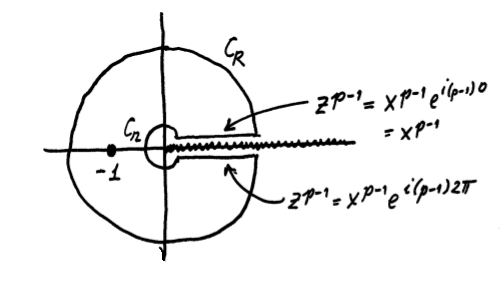
\includegraphics{figuras/15-1}
  \end{figure}
  \begin{dmath*}
    I(p) = \oint_C \frac{z^{p - 1}}{1 + z} \vi{z}.
  \end{dmath*}
  Como
  \begin{dmath*}
    z^{p - 1} = \exp\left( (p - 1) \ln z \right)
    = \exp\left( (p - 1) \left( \ln |z| + i (\theta + 2 \kappa \pi) \right) \right)
    = |z|^{p - 1} \exp\left( i (p - 1) (\theta + 2 k \pi \right).
  \end{dmath*}
  Podemos ainda notar que
  \begin{dgroup*}
    \begin{dmath*}
      \left| \int_{C_R} \left( \ldots \right) \right| \leq \int_0^{\infty}
      \frac{|r|^{p - 1} R}{R} \vi{\theta}
      \approx |R|^{p - 1}
      % TODO Quebrar linha aqui.
      \overset{R \to \infty}{\longrightarrow} 0 \condition{$p < 1$},
    \end{dmath*}
    \begin{dmath*}
      \left| \int_{C_R} \left( \ldots \right) \right| \leq \int_0^{\infty}
      \frac{|r|^{p - 1} r}{1 + r} \vi{r}
      \approx \int_0^{\infty} \frac{|r|^{p - 1} r}{r} \vi{r}
      \approx |r|^{-p}
      % TODO Quebrar linha aqui.
      \overset{R \to 0}{\longrightarrow} 0 \condition{$p > 0$}.
    \end{dmath*}
  \end{dgroup*}
  Então
  \begin{dmath*}
    2 \pi i \Res_{z = -1} f(z) = \int_r^R (\ldots) + \int_{C_R} (\ldots) +
    \int_R^r (\ldots) + \int_{C_R} (\ldots)
    = \lim_{r \to 0, R \to \infty} (\ldots)
    = \int_0^{\infty} (\ldots) + \int_{\infty}^0 (\ldots)
    = \int_0^{\infty} \frac{x^{p - 1}}{1 + x} \vi{x} + \int_{\infty}^0
    \frac{x^{p - 1} \exp(i (p - 1) 2 \pi)}{1 + x} \vi{x}
    = \left( 1 - \exp\left( i (p - 1) 2 \pi \right) \right) \int_0^{\infty}
    \frac{x^{p - 1}}{1 + x} \vi{x}
    = \exp\left( i (p - 1) \pi \right) \left( \exp\left( -i (p - 1) \pi \right)
    - \exp\left( i (p - 1) \pi \right)\right) \int_0^{\infty}
    \frac{x^{p - 1}}{1 + x} \vi{x}
    = \exp\left( i (p - 1) \pi \right) \left( -\exp\left( -i p \pi \right)
    + \exp\left( i p \pi \right)\right) \int_0^{\infty}
    \frac{x^{p - 1}}{1 + x} \vi{x}.
  \end{dmath*}
  Mas
  \begin{dmath*}
    \Res_{z = -1} f(z) = \lim_{z \to -1} (z + 1) \frac{z^{p - 1}}{1 + z}
    = (-1)^{p - 1}
    = \exp(i (p - 1) \pi)
  \end{dmath*}
  e, portanto,
  \begin{dmath*}
    2 \pi i \exp\left( i (p - 1) \pi \right) = e^{i (p - 1)} \left( \exp(i p
    \pi) - \exp(- i p \pi) \right) \int_0^{\infty} \frac{x^{p - 1}}{1 + x}
    \vi{x}.
  \end{dmath*}
  Conclui-se então que
  \begin{dmath*}
    \int_0^{\infty} \frac{x^{p - 1}}{1 + x} \vi{x} = F(p)
    = \pi / \sin(p \pi).
  \end{dmath*}

  Já para a transformada inversa:
  \begin{dmath*}
    f(x) = \frac{1}{2 \pi i} \int_{C - i \infty}^{C + i \infty}
    \frac{\pi}{\sin(p \pi)} x^{-p} \vi{p}
  \end{dmath*}
  onde os pólos simples em $p = k \pi$ para $k \in \mathbb{Z}$.
  \begin{figure}[htb]
    \centering
    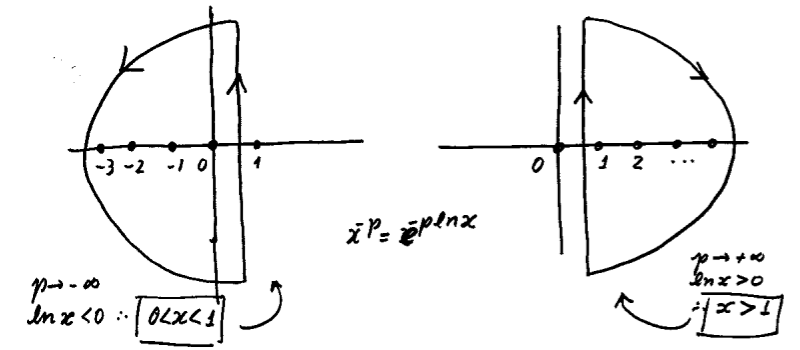
\includegraphics[width=.9\textwidth]{figuras/15-2}
  \end{figure}
  Então, se $0 < x < 1$,
  \begin{dmath*}
    f(x) = \sum_{k = 0}^{\infty} \Res_{p = - k} \left[ \frac{\pi x^{-p}}{\sin(p
    \pi)} \right]
    = \sum_{k = 0}^{\infty} \lim_{p \to -k} (p + k) \frac{\pi}{\sin(p \pi)}
    x^{-p}
    = \sum_{k = 0}^{\infty} \lim_{q \to 0} \frac{q \pi x^{-(q - k)}}{\sin\left(
    (q - k) \pi \right)}
    = \sum_{k = 0}^{\infty} \lim_{q \to 0} \frac{q \pi x^{-(q - k)}}{(-1)^k
    \sin(q \pi)}
    = \sum_{k = 0}^{\infty} \lim_{q \to 0} \frac{q \pi}{\sin(q \pi)} x^{-q}
    \frac{x^k}{(-1)^k}
    = \sum_{k = 0}^{\infty} (-x)^k
    = 1 / \left( 1 - (-x) \right)
    = 1 / (1 + x),
  \end{dmath*}
  se $x > 1$,
  \begin{dmath*}
    f(x) = - \sum_{k = 1}^{\infty} \Res_{p = k} \left[ \frac{\pi x^{-p}}{\sin(p
    \pi)} \right]
    = - \sum_{k = 1}^{\infty} \lim_{p \to k} \frac{(p - k) \pi x^{-p}}{\sin(p
    \pi)}
    = - \sum_{k = 1}^{\infty} \lim_{q \to 0} \frac{q \pi x^{- (1 +
    k)}}{\sin\left( (q + k) \pi \right)}
    = - \sum_{k = 1}^{\infty} \lim_{q \to 0} \frac{q \pi x^{- (1 +
    k)}}{(-1)^k \sin(q \pi)}
    = - \sum_{k = 1}^{\infty} \lim_{q \to 0} \frac{q \pi}{\sin(q \pi)} x^{-q}
    \frac{x^{-k}}{(-1)^k}
    = - \sum_{k = 1}^{\infty} (-x^{-q})^k
    = - \left[ \sum_{k = 0}^{\infty} (-x^{-1})^k - 1 \right]
    = - \left[ \frac{1}{1 + x^{-1}} - 1 \right]
    = - \left[ \frac{1 - 1 - x^{-1}}{1 + x^{-1}} \right]
    = x^{-1} / \left( 1 + x^{-1} \right)
    = 1 / \left( x + 1 \right),
  \end{dmath*}
  e se $x = 1$,
  \begin{dmath*}
    f(1) = \frac{1}{2 \pi i} \int_{-i \infty}^{+i \infty} \frac{\pi}{\sin(p
    \pi)} \vi{p}
    = \frac{1}{2 \pi i} \lim_{R \to \infty} \int_{-i R}^{+i R}
    \frac{1}{\sin(p \pi)} \vi{(p \pi)}
    = \frac{1}{2 \pi i} \lim_{R \to \infty} \left. \left[ \ln \tan(p \pi / 2)
    \right] \right|_{-i R}^{+i R}
    = \frac{1}{2 \pi i} \lim_{R \to \infty} \left[ \ln \tan(i R \pi / 2) - \ln
    \tan(-i R \pi / 2) \right]
    = \frac{1}{2 \pi i} \lim_{R \to \infty} \ln \left[ \frac{\tan(i R \pi /
    2)}{\tan(- i R \pi / 2)} \right]
    = \frac{1}{2 \pi i} \lim_{R \to \infty} \ln \left[ \frac{\tan(i R \pi /
    2)}{- \tan(i R \pi / 2)} \right]
    = \frac{1}{2 \pi i} \ln(-1)
    = \frac{1}{2 \pi i} \ln\left( \exp(i \pi) \right)
    = \frac{1}{2 \pi i} i \pi
    = 1/2
  \end{dmath*}

  Conclusão, $f(x) = 1 / (1 + x)$.
\end{exem}

Para estudar algumas propriedades da transformada de Mellin, vamos usar uma
notação apropriada:
\begin{dmath*}
  \mathcal{M}[f](p) = \int_0^{\infty} f(x) x^{p - 1} \vi{x}.
\end{dmath*}

Algumas das propriedades mais importantes das transformadas de Mellin são:
\begin{dgroup*}
  \begin{dmath*}
    \mathcal{M}[x^{\alpha} f(x)](p) = \mathcal{M}[f(x)](p + \alpha),
  \end{dmath*}
  \begin{dmath*}
    \mathcal{M}[f'(x)](p) = -(p - 1) \mathcal{M}[f(x)](p - 1),
  \end{dmath*}
  \begin{dmath*}
    M[x f'(x)](p) = -p \mathcal{M}[f(x)](p),
  \end{dmath*}
  \begin{dmath*}
    M[x^n f^{(n)}(x)](p) = (-1)^n (p)_n \mathcal{M}[f(x)](p),
  \end{dmath*}
\end{dgroup*}
onde usamos o símbolo de Pochhammer, $(p)_n = p (p + 1) \ldots (p + n - 1)$.
Quanto à demonstração, a da primeira é óvia. Já a segunda se faz por partes,
sendo que observamos que devemos supor $\lim_{x \to 0} f(x) x^{p - 1} = 0$ para
$\Re(p) > \alpha$ e $\lim_{x \to \infty} f(x) x^{p - 1} = 0$ para $\Re(p) <
\beta$, sendo que $\mathcal{M}[f(x)](p)$ existe para $\alpha < \Re(p) < \beta$.
A terceira e a quarta sequem usando essas duas primeiras propriedades.

Quanto à propriedades de convolução, precisamos adaptar a sua definição para a
transformada de Mellin. Como passamos de Fourier para Mellin através da mudança
de variável $x = \exp(t)$, vamos fazer essa mudança na definição da convolução
dentro do contexto das transformadas de Fourier. Tomando $x = \exp(t)$ e
$\epsilon = \exp(\tau)$ temos
\begin{dmath*}
  \int_{-\infty}^{+\infty} f(\tau) g(t - \tau) \vi{\tau} = \int_0^{\infty} f(\ln
  \epsilon) g(\ln x - \ln \epsilon) (1 / \epsilon) \vi{\epsilon}
  = \int_0^{\infty} \epsilon^{-1} F(\epsilon) G(x / \epsilon) \vi{\epsilon}.
\end{dmath*}

Portanto, dentro do contexo das transformadas de Mellin, definimos a convolução
como
\begin{dmath*}
  (f * g)(x) = \int_0^{\infty} \epsilon^{-1} f(\epsilon) g(x / \epsilon)
  \vi{\epsilon}.
\end{dmath*}
Agora:
\begin{dmath*}
  \mathcal{M}[(f * g)(x)] = \int_0^{\infty} x^{p - 1} \int_0^{\infty}
  \epsilon^{-1} f(\epsilon) g(x / \epsilon) \vi{\epsilon} \vi{x}
  = \int_0^{\infty} \int_0^{\infty} x^{p - 1} \epsilon^{-1} f(\epsilon) g(x /
  \epsilon) \vi{\epsilon} \vi{x}
  = \int_0^{\infty} \int_0^{\infty} \epsilon (\epsilon y)^{p - 1} \epsilon^{-1}
  f(\epsilon) g(y) \vi{\epsilon} \vi{y}
  = \int_0^{\infty} y^{p - 1} g(y) \int_0^{\infty} \epsilon^{p - 1} f(\epsilon)
  \vi{\epsilon} \vi{y}
  = \mathcal{M}[f](p) \mathcal{M}[g](p)
\end{dmath*}
de modo que, com essa definição de convolução, temos
\begin{dmath*}
  \mathcal{M}[(f * g)(x)](p) = \mathcal{M}[f(x)](p) \mathcal{M}[g(x)](x).
\end{dmath*}

Outra propriedade a considerar envolve a transformada $\mathcal{M}[f(x \exp(i
\theta))]$. Temos
\begin{dmath*}
  \mathcal{M}[f(x \exp(i \theta))](p) = \int_0^{\infty} x^{p - 1} f(x \exp(i
  \theta)) \vi{x}
  = \exp(- i \theta p) \int_C y^{p - 1} f(y) \vi{y},
\end{dmath*}
onde tomamos $y = x \exp(i \theta)$. Visto que a operação $z \to z \exp(i
\theta)$ é uma rotação por um ângulo $\theta$ no plano complexo, o caminho $C$ é
o limite do caminho $C_R$ abaixo para $R \to \infty$. Se $f(y)$ é analítica na
região limitada pelas curvas abaixo, temos
\begin{figure}[htb]
  \centering
  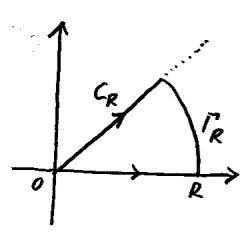
\includegraphics{figuras/15-3}
\end{figure}
\begin{dmath*}
  \oint = 0 \hiderel{=} - \int_{C_R} + \int_0^R + \int_{\Gamma_R}.
\end{dmath*}
Em $\Gamma_R$ temos $y = R \exp(i \theta)$, $\vi{y} = R \exp(i \theta) i
\vi{\theta}$ e
\begin{dmath*}
  \int_{\Gamma_R} R \exp(i \theta) \left( R \exp(i \theta) \right)^{p - 1}
  f\left( R \exp(i \theta) \right) i \vi{\theta} = \int_{\Gamma_R} \exp(i \theta
  p) R^p f(R \exp(i \theta) i \vi{\theta},
\end{dmath*}
ou seja,
\begin{dmath*}
  \int_{\Gamma_R} \overset{R \to \infty}{\longrightarrow} 0 \condition{se $R^p
  f(R) \overset{R \to \infty}{\longrightarrow} 0$}.
\end{dmath*}
Com essa hipótese, temos $\int_C = \int_0^{\infty}$ e portanto
\begin{dmath*}
  \mathcal{M}[f(x \exp(i \theta))](p) = \exp(-i \theta p) \mathcal{M}[f(x)](p)
\end{dmath*}
ou ainda
\begin{dgroup*}
  \begin{dmath*}
    cos(\theta p) \mathcal{M}[f(x)](p) = \Re[\mathcal{M}[f(x \exp(i \theta))]](p)
  \end{dmath*}
  \begin{dmath*}
    \sin(\theta p) \mathcal{M}[f(x)](p) = -\Im[\mathcal{M}[f(x \exp(i \theta))]](p).
  \end{dmath*}
\end{dgroup*}

\begin{exem}
  Já vimos que
  \begin{dmath*}
    \mathcal{M}[1 / (1 + x)] = \pi / \sin(p \pi).
  \end{dmath*}
  Agora vamos verificar que
  \begin{dmath*}
    \mathcal{M}[H(Q - x)] = \int_0^{\infty} x^{p - 1} H(a - x) \vi{x}
    = \int_0^{\alpha} x^{p - 1} \vi{x}
    = a^p / p \condition{$p > 0$}.
  \end{dmath*}
  Então temos a convolução:
  \begin{dmath*}
    \int_0^{\infty} \epsilon^{-1} H(a - \epsilon) \frac{1}{1 + x / \epsilon}
    \vi{\epsilon} = \int_0^a \epsilon^{-1} \frac{\epsilon}{\epsilon + x}
    \vi{\epsilon}
    = \left. \ln(\epsilon + x) \right|_0^a
    = \ln\left( (x + a) / x \right).
  \end{dmath*}
  Portanto,
  \begin{dmath*}
    \mathcal{M}[\ln(1 + a / x)] = \frac{a^p}{p} \frac{\pi}{\sin(p \pi)}.
  \end{dmath*}
\end{exem}

\begin{exem}
  Considere
  \begin{dmath*}
    \mathcal{M}[1 / (1 + x^a)] = \int_0^{\infty} \frac{x^{p - 1}}{1 + x^a}
    \vi{x}
    = \frac{1}{a} \int_0^{\infty} \frac{y^{p / a - 1}}{1 + y} \vi{y}
    = \frac{1}{a} \frac{\pi}{\sin(p \pi / a)}.
  \end{dmath*}
  Então
  \begin{dmath*}
    \mathcal{M}[f(x \exp(i \theta))] = \int_0^{\infty} \frac{x^{p - 1}}{1 + (x
    (\exp(i \theta))^a} \vi{x}
    = \int_0^{\infty} \frac{x^{p - 1}}{1 + x^a \exp(i \theta a)} \vi{x}
    = \int_0^{\infty} \frac{x^{p - 1}}{1 + x^a \cos(\theta a) + i x^a
    \sin(\theta a)} \vi{x}
    = \int_0^{\infty} \frac{x^{p - 1} (1 + x^a \cos(\theta a) - i x^a
    \sin(\theta a)}{(1 + x^a \cos(\theta a))^2 + (x^a \sin(\theta a))^2}
    = \int_0^{\infty} \frac{x^{p - 1}(1 + x^a \cos(\theta a) - i x^a \sin(\theta
    a)}{1 + 2 x^a \cos(\theta a) + x^{2 a}} \vi{x}
    = \exp(-i p \theta) \int_0^{\infty} \frac{x^{p - 1}}{1 + x^a} \vi{x}
    = \exp(-i p \theta) \frac{\pi}{a \sin(p \pi / a)}.
  \end{dmath*}
  Logo,
  \begin{dgroup*}
    \begin{dmath*}
      \cos(\theta p) \frac{\pi}{a \sin(p \pi /a} = \mathcal{M}\left[ \frac{1 +
      x^a \cos(\theta a)}{1 + 2 x^a \cos(\theta a) + x^{2 a}} \right]
    \end{dmath*}
    \begin{dmath*}
      \sin(\theta p) \frac{\pi}{a \sin(p \pi / a)} = \mathcal{M}\left[ \frac{x^a
      \sin(\theta a)}{1 + 2 x^a \cos(\theta a) + x^{2 a}} \right]
    \end{dmath*}
  \end{dgroup*}
\end{exem}

% TODO Adicionar o exemplo que inicia-se na página 2 de M2S12-16.pdf

\section{Transformada de Hankel}
Vamos considerar uma função de duas variáveis $f(x, y)$ e a sua transformada de
Fourier $F(K, L)$, ou seja,
\begin{dgroup*}
  \begin{dmath*}
    F(K, L) = \frac{1}{2 \pi} \int_{-\infty}^{+\infty} \int_{-\infty}^{+\infty}
    f(x, y) \exp\left( i (K x + L y) \right) \vi{y} \vi{x},
  \end{dmath*}
  \begin{dmath*}
    f(x, y) = \frac{1}{2 \pi} \int_{-\infty}^{+\infty} F(K, L) \exp\left( i (K x
    + L y) \right) \vi{L} \vi{K}.
  \end{dmath*}
\end{dgroup*}
Agora vamos passar apra coordenadas polares. Por abuso de notação, vamos denotar
$f(r, \theta) = f(x(r, \theta), y(r, \theta))$ e $F(\rho, \varphi) = F(K(\rho,
\varphi), L(\rho, \varphi))$. Uma vez que essas funções tem periodicidade
angular, ou seja, temos $f(r, \theta + 2 \pi) = f(r, \theta)$ e $F(\pi, \varphi
+ 2 \pi) = F(\rho, \varphi)$, podemos nessa variável tomar uma séria de Fourier,
de modo que
\begin{dgroup*}
  \begin{dmath}
    f(r, \theta) = \sum_{n = -\infty}^{+\infty} f_n(r) \exp(i n \theta),
  \end{dmath}
  \begin{dmath*}
    f_n(r) = \frac{1}{2 \pi} \int_0^{2 \pi} f(r, \theta) \exp(-i n \theta)
    \vi{\theta},
  \end{dmath*}
  \begin{dmath*}
    F(\rho, \varphi) = \sum_{n = -\infty}^{+\infty} F_n(\rho) \exp(i n \varphi),
  \end{dmath*}
  \begin{dmath*}
    F_n(\rho) = \frac{1}{2 \pi} \int_0^{2 \pi} F(\rho, \varphi) \exp(-i n
    \varphi) \vi{\varphi}.
  \end{dmath*}
\end{dgroup*}
Em coordenadas polares temos
\begin{dmath*}
  F(\rho, \varphi) = \frac{1}{2 \pi} \int_0^{\infty} r \int_0^{2 \pi} f(r,
  \theta) \exp\left(i \left[ (\rho \cos\varphi) (r \cos\theta) + (\rho \sin\varphi)
  (r \sin\theta) \right] \right) \vi{\theta} \vi{r}
  = \frac{1}{2 \pi} \int_0^{\infty} r \int_0^{2 \pi} f(r, \theta) \exp(i p r
  \cos(\varphi - \theta)) \vi{\theta} \vi{r}
\end{dmath*}
e portanto
\begin{dmath*}
  F_n(\rho) = \frac{1}{2 \pi} \int_0^{2 \pi} \exp(-i n \varphi)
  \frac{1}{2 \pi} \int_0^{\infty} r \int_0^{2 \pi} f(r, \theta) \exp(i \rho r
  \cos(\varphi - \theta)) \vi{\theta} \vi{r} \vi{\varphi}
  = \frac{1}{(2 \pi)^2} \int_0^{\infty} r \int_0^{2 \pi} \int_0^{2 \pi} \exp(-i
  n \varphi) \exp(i \rho r \cos(\varphi - \theta)) \sum_{m = -\infty}^{+\infty}
  f_m(r) \exp(i m \theta) \vi{\theta} \vi{\varphi} \vi{r}
  = \frac{1}{(2 \pi)^2} \int_0^{\infty} r \sum_{m = -\infty}^{+\infty} f_m(r)
  \int_0^{2 \pi} \int_0^{2 \pi} \exp(-i n (\alpha + \theta)) \exp(i \rho r
  \cos(\alpha)) \exp(i m \theta) \vi{\theta} \vi{\alpha} \vi{r}
\end{dmath*}
onde usamos, na integração em $\alpha$, o fato da periodicidade ser $2 \pi$, o
que implica que $\int_{0 + \theta}^{2 \pi + \theta} (\ldots) \vi{\alpha} =
\int_0^{2 \pi} (\ldots) \vi{\alpha}$. Continuando:
\begin{dmath*}
  F_n(\rho) = \frac{1}{2 \pi} \int_0^{\infty} r \sum_{m = -\infty}^{+\infty}
  f_m(r) \int_0^{2 \pi} \exp(-i n \alpha) \exp(i p r \cos\alpha)
  \frac{1}{2 \pi} \int_0^{2 \pi} \exp(-i n \theta) \exp(i m \theta) \vi{\theta}
  \vi{\alpha} \vi{r}
  = \frac{1}{2 \pi} \int_0^{\infty} r \sum_{m = -\infty}^{+\infty}
  f_m(r) \int_0^{2 \pi} \exp(-i n \alpha) \exp(i p r \cos\alpha)
  \sigma_{mn} \vi{\alpha} \vi{r}
  = \frac{1}{2 \pi} \int_0^{\infty} r f_n(r) \int_0^{2 \pi} \exp(-i r \alpha)
  \exp(i \rho r \cos\alpha) \vi{\alpha} \vi{r}.
\end{dmath*}
Mas a função geratriz para as funções de Bessel é
\begin{dmath*}
  \exp\left( z (t - 1/t) / 2 \right) = \sum_{n = -\infty}^{+\infty} t^n J_n(z),
\end{dmath*}
ou, tomando $t = i \exp(i \varphi)$
\begin{dmath*}
  \exp(i z \cos\varphi) = \sum_{n = -\infty}^{+\infty} i^n \exp(i n \varphi)
  J_n(z)
\end{dmath*}
de modo que
\begin{dmath*}
  \frac{1}{2 \pi} \int_0^{2 \pi} \exp(-i n \varphi) \exp(i z \cos\varphi) = i^n
  J_n(z)
\end{dmath*}
e portanto
\begin{dmath*}
  F_n(\rho) = \int_0^{\infty} r f_n(r) i^n J_n(\rho r) \vi{r}.
\end{dmath*}
De modo análogo:
\begin{dmath*}
  f_n(r) = \frac{1}{2 \pi} \int_0^{2 \pi} \exp(-i n \theta)
  \frac{1}{2 \pi} \int_0^{\infty} \rho \int_0^{2 \pi} F(\rho, \varphi) \exp\left(-i
  \rho r \cos(\theta - \varphi) \right) \vi{\varphi} \vi{\rho} \vi{\theta}
  = \frac{1}{2 \pi} \int_0^{\infty} \rho \int_0^{2 \pi} \exp(-i n \alpha)
  \exp(-i \rho r \cos\alpha) \sum_{m = -\infty}^{+\infty} F_m(\rho)
  \frac{1}{2 \pi} \int_0^{2 \pi} \exp(-i n \varphi) \exp(i m \varphi)
  \vi{\varphi} \vi{\alpha} \vi{\rho}
  = \frac{1}{2 \pi} \int_0^{\infty} \rho \int_0^{2 \pi} \exp(-i n \alpha)
  \exp(-i \rho r \cos\alpha) \sum_{m = -\infty}^{+\infty} F_m(\rho)
  \sigma_{mn} \vi{\alpha} \vi{\rho}
  = \int_0^{\infty} \rho F_n(\rho) \frac{1}{2 \pi} \int_0^{2 \pi} \exp(-i r
  \alpha) \exp(-i \rho r \cos\alpha) \vi{\alpha} \vi{\rho}
  = \int_0^{\infty} \rho F_n(\rho) (-i)^n J_n(\rho r) \vi{\rho}.
\end{dmath*}
Resumindo, temos:
\begin{dgroup*}
  \begin{dmath*}
    F_n(\rho) = i^n \int_0^{\infty} r J_n(\rho r) f_n(r) \vi{r},
  \end{dmath*}
  \begin{dmath*}
    f_n(r) = (-i)^n \int_0^{\infty} \rho J_n(\rho r) F_n(\rho) \vi{\rho},
  \end{dmath*}
\end{dgroup*}
o que nos sugere definir a transformada de Hankel de ordem $\nu$,
$\mathcal{H}_{\nu}$, e sua inversa, $\mathcal{H}_{\nu}^{-1}$ como
\begin{dgroup*}
  \begin{dmath*}
    \mathcal{H}_{\nu}[f(x)] = \int_0^{\infty} x J_{\nu}(K x) f(x) \vi{x}
    \hiderel{=} F_{\nu}(K),
  \end{dmath*}
  \begin{dmath*}
    \mathcal{H}_{\nu}^{-1}[F_{\nu}(K)] = \int_0^{\infty} K J_{\nu}(K x)
    F_{\nu}(K) \vi{K} \hiderel{=} f(x).
  \end{dmath*}
\end{dgroup*}

\begin{exem}
  Vamos calcular $\mathcal{H}_0[\exp(-\alpha x)]$.
  \begin{dmath*}
    \mathcal{H}[\exp(-\alpha x)] = \int_0^{\infty} x J_0(K x) \exp(-\alpha x)
    \vi{x}
    = \sum_{n = 0}^{\infty} \frac{(-1)^n K^{2n}}{2^{2n} (n!)^2} \int_0^{\infty}
    x^{2 n + 1} \exp(-\alpha x) \vi{x}
    = \sum_{n = 0}^{\infty} \frac{(-1)^n K^{2 n}}{2^{2 n} (n!)^2}
    \frac{\Gamma(2 n + 2)}{a^{2 n + 2}}
  \end{dmath*}
  mas da fórmula de duplicação de Legendre,
  \begin{dmath*}
    \sqrt{\pi} \Gamma(2 z + 1) = 2^{2 z} \Gamma(z + 1 / z) \Gamma(z + 1),
  \end{dmath*}
  temos
  \begin{dmath*}
    \Gamma(2 n + 1) = \Gamma\left[ 2 (n + 1 / 2) + 1 \right]
    = \frac{2^{2 (n + 1 / 2)}}{\sqrt{\pi}} \Gamma\left[ 1 + (1/2) + (1/2)
    \right] \Gamma\left[ n + (1/2) + 1 \right]
  \end{dmath*}
  e portanto
  \begin{dmath*}
    \mathcal{H}_0[\exp(-\alpha x)] = \sum_{K = 0}^{\infty} \frac{(-1)^n K^{2
    n}}{2^{2 n} [\Gamma(n + 1)]^2} \frac{2^{2 n} 2}{\sqrt{\pi}}
    \frac{\Gamma(n + 1) \Gamma(n + 3 / 2}{\alpha^{2 n + 2}}
    = \frac{1}{\alpha^2} \sum_{n = 0}^{\infty} \frac{(-1)^n (K / \alpha)^{2
    n}}{\Gamma(n + 1)} \frac{\Gamma(n + 3/2)}{\Gamma(3/2)}
    = \frac{1}{a^2} \sum_{n = 0}^{\infty} \frac{(-1)^n (K / \alpha)^{2
    n}}{\Gamma(n + 1)} \frac{\Gamma(n + 3/2)}{\sqrt{\pi} / 2}
    = \frac{1}{\alpha^2} \sum_{n = 0}^{\infty} (-1)^n (3/2)_n
    \frac{[(k/\alpha)^2]^n}{n!}
    = \frac{1}{\alpha^2} \frac{1}{[1 + (x / \alpha)^2]^{3/2}}
    = \frac{a}{(\alpha^2 + x^2)^{3/2}}.
  \end{dmath*}
\end{exem}

Uma das propriedades que mais nos interessa no caso de uma transformada integral
envolve a derivada de uma função. Nesse caso temos
\begin{dmath*}
  \mathcal{H}_{\nu}[f'(x)] = \int_0^{\infty} x J_{\nu}(K x) f'(x) \vi{x}
  = \left. x J_{\nu}(K x) f(x) \right|_0^{\infty} - \int_0^{\infty} \left[ x
  J_{\nu}(K x) \right]' f(x) \vi{x}
  = - \int_0^{\infty} \left[ x J_{\nu}(K x) \right]' f(x) \vi{x} \condition{se
  $\lim_{x \to \infty} f(x) = 0$.}
\end{dmath*}
Sabemos, porém, que
\begin{dgroup*}
  \begin{dmath*}
    2 J_{\nu}'(x) = J_{\nu - 1}(x) - J_{\nu + 1}(x),
  \end{dmath*}
  \begin{dmath*}
    \nu J_{\nu}(x) = \frac{x}{2} J_{\nu + 1}(x) + \frac{x}{2} J_{\nu - 1}(x)
  \end{dmath*}
\end{dgroup*}
Logo:
\begin{dmath*}
  (x J_{\nu}(x))' = J_{\nu}(x) + x J_{\nu}'(x)
  = \frac{x}{2 \nu} \left( J_{\nu + 1}(x) + J_{\nu - 1}(x) \right) +
  \frac{x}{2} \left( J_{\nu - 1}(x) - J_{\nu + 1}(x) \right)
  = \frac{x}{2} J_{\nu + 1}(x) \left( \frac{1 - \nu}{\nu} \right) +
  \frac{x}{2} J_{\nu - 1}(x) \left( \frac{1 + \nu}{\nu} \right).
\end{dmath*}
Sendo assim
\begin{dmath*}
  \mathcal{H}_{\nu}[f'(x)] = - K \int_0^{\infty} \left[ \frac{x}{2} J_{\nu +
  1}(K x) \left( \frac{1 - \nu}{\nu} \right) + \frac{x}{2} J_{\nu - 1}(K x)
  \left( \frac{1 + \nu}{\nu} \right) \right] f(x)
  = -K \left( \frac{1 - \nu}{2 \nu} \right) \mathcal{H}_{\nu + 1}[f(x)] - K
  \left( \frac{1 + \nu}{2 \nu} \right) \mathcal{H}_{\nu - 1}[f(x)]
  \condition{$\nu \geq 1$.}
\end{dmath*}
Não é, porém, nesse caso que a transformada de Hankel assume seu papel mais
simples. De fato, temos
\begin{dmath*}
  \mathcal{H}_{\nu}\left[ f''(x) + \frac{1}{x} f'(x) - \frac{\nu^2}{x^2} f(x)
  \right] = \int_0^{\infty} \left[ f''(x) + \frac{1}{x} f'(x) -
  \frac{\nu^2}{x^2} f(x) \right] J_{\nu}(K x) x \vi{x}
  = \left. f'(x) J_{\nu}(K x) x \right|_0^{\infty} + \left. f(x) J_{\nu}(K x)
  \right|_0^{\infty} + \int_0^{\infty} \left[ -f'(x) \left( J_{\nu}(K x) x
  \right)' - f(x) J_{\nu}' (K x) - \frac{\nu^2}{x} f(x) J_{\nu}(K x) \right]
  \vi{x}
  = \int_0^{\infty} \left[ -f'(x) \left( J_{\nu}(K x) x \right)' - f(x) J_{\nu}'
  (K x) - \frac{\nu^2}{x} f(x) J_{\nu}(K x) \right] \vi{x}
  = \left. -f(x) \left( J_{\nu}(K x) x \right)' \right|_0^{\infty} +
  \int_0^{\infty} \left[ f(x) \left( J_{\nu}(K x) x \right)'' - f(x) J_{\nu}'(K
  x) - \frac{\nu^2}{x} f(x) J_{\nu}(K x) \right] \vi{x}
  = \int_0^{\infty} \left[ f(x) \left( J_{\nu}(K x) x \right)'' - f(x) J_{\nu}'(K
  x) - \frac{\nu^2}{x} f(x) J_{\nu}(K x) \right] \vi{x}
  = \int_0^{\infty} \left[ f(x) \left( J_{\nu}'(K x) x + J_{\nu}(K x) \right)' -
  f(x) J_{\nu}'(K x) - \frac{\nu^2}{x} f(x) J_{\nu}(K x) \right] \vi{x}
  = \int_0^{\infty} \left[ f(x) \left( J_{\nu}''(K x) x + 2 J_{\nu}'(K x)
  \right) - f(x) J_{\nu}'(K x) - \frac{\nu^2}{x} f(x) J_{\nu}(K x) \right]
  \vi{x}
  = \int_0^{\infty} \left[ f(x) J_{\nu}''(K x) x + 2 f(x) J_{\nu}'(K x) - f(x)
  J_{\nu}'(K x) - \frac{\nu^2}{x} f(x) J_{\nu}(K x) \right] \vi{x}
  = \int_0^{\infty} f(x) x \left[ J_{\nu}''(K x) + (1 / x) J_{\nu}'(K x) -
  \frac{\nu^2}{x^2} J_{\nu}(K x) \right] \vi{x}
\end{dmath*}
mas, da equação de Bessel para $z = K x$, segue que
\begin{dmath*}
  J_{\nu}''(K x) + J_{\nu}'(K x) + \left( K^2 - \frac{\nu^2}{x^2} \right)
  J_{\nu}(K x) = 0
\end{dmath*}
e portanto
\begin{dmath*}
  \int_0^{\infty} f(x) x \left[ J_{\nu}''(K x) + (1 / x) J_{\nu}'(K x) -
  \frac{\nu^2}{x^2} J_{\nu}(K x) \right] \vi{x} = \int_0^{\infty} f(x) \left[
  -K^2 J_{\nu}(K x) \right] x \vi{x}
  = -K^2 \mathcal{H}_{\nu}[f(x)].
\end{dmath*}

% TODO Adicionar exemplo da página 11 de M2S12-16.pdf
